\documentclass{beamer}
\usepackage[latin1]{inputenc}
\usepackage{color}
\usepackage{multirow}
%\usepackage[pdftex]{graphicx}
%\usepackage{sidecap}
%\usepackage{siunitx}
%\usepackage{epstopdf}
\usetheme{default}
\title{Long Baseline Neutrino Facility \\ (for the comprehensive exam)}
\author{Ekaterina Avdeeva}
\institute{University of Nebraska - Lincoln}
\date{May 4th, 2015}

\begin{document}

\begin{frame}
\titlepage
\end{frame}

\begin{frame}
  \frametitle{Outline}
  \scriptsize
  \begin{itemize}
    \scriptsize
    \item Introduction. Neutrinos in the Standard Model
    \item Neutrino Oscillations Overview
      \begin{itemize}
         \scriptsize
         \item Discovery
         \item Theory
         \item Current Status
      \end{itemize}   
    \scriptsize
    \item Experimental Setup of the LBNF
      \begin{itemize}
         \scriptsize
         \item Beam Production System
         \item Near Detector
         \item Far Detector
         \item Comparison to the Other Facilities
      \end{itemize}  
    \scriptsize 
    \item Conclusions
  \end{itemize}
\end{frame}

\begin{frame}\frametitle{Introduction. Standard Model}
\begin{figure}
\label{fig:StandardModel}
\centering 
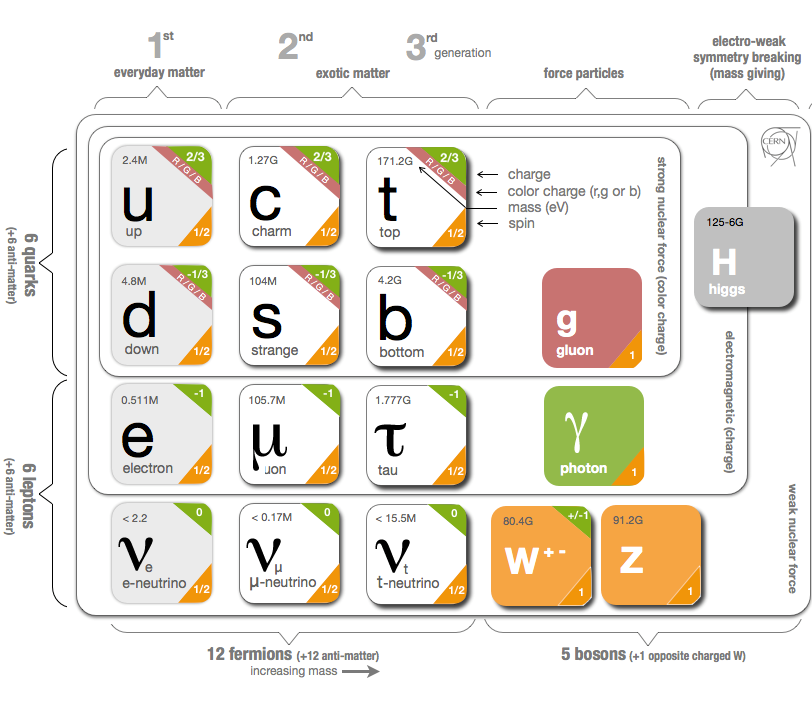
\includegraphics[width=0.75\textwidth, keepaspectratio=true]{figs/StandardModel.png}
\end{figure}
\tiny
All these and only these fundamental particles are discovered at the moment. Source of picture: \cite{ref_fig_StandardModel}
\end{frame}

\begin{frame}\frametitle{Introduction. Neutrino Interactions}
\scriptsize
Feynmann diagrams of neutral current (NC, left), and neutral current (CC, middle and right) neutrino scattering.
\begin{figure}
\label{fig:NuScattering}
\centering
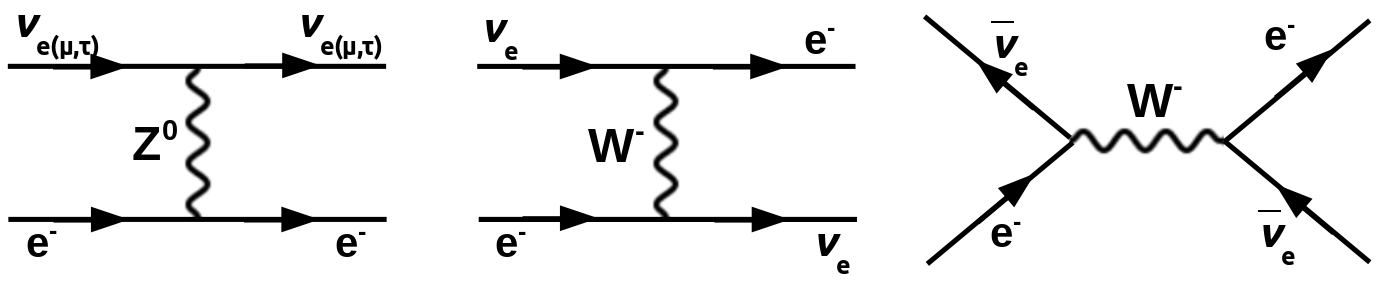
\includegraphics[width=0.90\textwidth, keepaspectratio=true]{figs/neutrinoScattering.png}
\end{figure}
Quoting \cite{ref_Griffiths}, 11.1: "John Bahcall, who was responsible for most of the calculations of solar neutrino abundances, liked to say that 100 billion neutrinos pass through your thumbnail every second; and yet they are so ethereal that you can look forward to only one or two neutrino-induced reaction in your body during your entire lifetime".\\
\end{frame}

\begin{frame}\frametitle{Introduction. Cosmic shower}
\begin{figure}
\caption{Cosmic shower induced by scattering of the incident cosmics proton of an air molecule. Charged and neutron pions are born in the reaction and then they further decay as $\pi^0 \rightarrow \gamma\gamma$, $\pi^+ \rightarrow \mu^+ + \nu_\mu$, $\pi^- \rightarrow \mu^- + \bar{\nu_\mu}$.}
\label{fig:cosmicMuons}
\centering
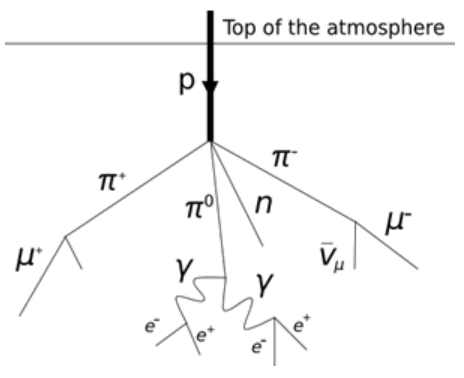
\includegraphics[width=0.60\textwidth, keepaspectratio=true]{figs/cosmicMuons.png}
\end{figure}
\end{frame}

\begin{frame}\frametitle{Introduction. Muon and Neutron Decay}
\scriptsize
\begin{figure}
\caption{Feynmann diagrams of (left) neutron and (right) muon decays. Neutron beta decay \cite{ref_fig_NeutronDecay}(d-quark of transfers to u-quark through the W-boson with emission of electron and antineutrino). Muon decay \cite{ref_fig_MuonDecay}(muon decays to electron, neutrino and antineutrino through W-boson}
\label{fig:MuonAndNeutronDecays}
\centering
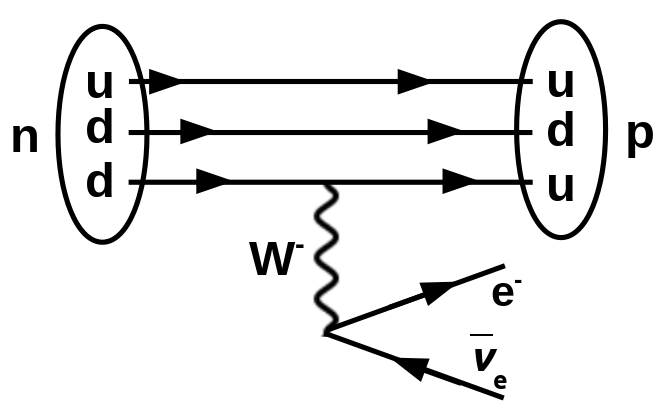
\includegraphics[width=0.35\textwidth, keepaspectratio=true]{figs/NeutronBetaDecay.png}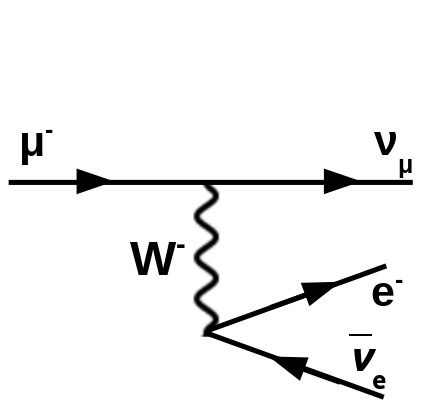
\includegraphics[width=0.35\textwidth, keepaspectratio=true]{figs/MuonDecay.png}
\end{figure}
\end{frame}

\begin{frame}\frametitle{Introduction. Lepton Flavor Number}
\scriptsize
3 flavors of neutrino, one for each generation: $\nu_e$, $\nu_\mu$, $\nu_\tau$. 3 lepton flavor numbers: $L_e$, $L_{\mu}$ and $L_{\tau}$ 

\begin{table}[h]
  \begin{center}
  \caption{ Lepton Flavor Number}
  \begin{tabular}{|c|c|c|c|}
     particles & $L_e$ & $L_{\mu}$ & $L_{\tau}$ \\ \hline
     $e^-,\nu_e$ &  +1  &  0  &  0  \\ \hline 
     $e^+, \bar{\nu_e}$ &  -1  &  0  &  0  \\ \hline 
     $\mu^-,\nu_{\mu}$ &  0  &  +1  &  0  \\ \hline 
     $\mu^+, \bar{\nu_{\mu}}$ &  0  &  -1  &  0  \\ \hline 
     $\tau^-,\nu_{\tau}$ &  0  &  0  &  +1  \\ \hline 
     $\tau^+, \bar{\nu_{\tau}}$ &  0  &  0  &  -1  \\ \hline 
  \end{tabular}
  \label{tab:LeptonFlavorNumber}
  \end{center}
\end{table}
\scriptsize
The lepton flavor numbers are conserved in almost all particle physics processes and the only violation of this law observed by this time is the neutrino oscillations - the ability of neutrino to change flavor. 
\end{frame}

\begin{frame}\frametitle{Neutrino Oscillations Discovery}
%\scriptsize
%History of the neutrino oscillations discovery is described in the Griffiths textbook \cite{ref_Griffiths}, chapter 11.
%\begin{itemize}
%  \scriptsize
%  \item Homestake experiment, 1968
%  \tiny
%  \begin{itemize}
%     \item Chlorino radiochemical detector ($\nu_e + ^{37}Cl \rightarrow ^{37}Ar+e$) 
%     \item Sensitive to $\nu_e$ only 
%     \item Recorded $1/3$ of theoretically predicted neutrino flux
%     \item Solar neutrino problem postulated
%  \end{itemize}
%  \scriptsize
%  \item Bruno Pontecorvo proposes theory: neutrino can change flavor and thus $\nu_e$ converted to $\nu_\mu$ and/or $\nu_\tau$ and weren't registered. But at first it was believed the Homestake experiment made mistake
%  \item more neutrino experiments report lack of Sun electron neutrinos
%  \item Super-Kamiokande experiment, 1998 
%  \tiny
%  \begin{itemize}
%     \item Water Cherenkov detector ($\nu + e \rightarrow \nu + e$). 
%     \item Sensitive to all $\nu$ but detection efficency of $\nu_e$ is 6.5 times bigger
%     \item Recorded $45\%$ of theoretically predicted neutrino flux (assumed all $\nu$=$\nu_e$)
%  \end{itemize}
%  \scriptsize
%  \item Solar neutrino observatory (SNO), 2002
%  \tiny
%  \begin{itemize}
%     \item Heavy water Cherenkov detector ($\nu_e + d \rightarrow p+p+e$, $\nu+d \rightarrow n+p+\nu$, $\nu+e \rightarrow \nu+e$)
%     \item Sensitive to all $\nu$ but can separate $\nu_e$
%     \item Reported $\nu_e$ flux to be $35\%$ of the predicted flux
%  \end{itemize}
%  \scriptsize
%  \item Combining Super-Kamiokande and SNO results
%  \tiny
%  \begin{itemize}
%     \item $45\%=35\%+10\%$, $10\% \cdot 6.5 = 65\%$, $35\%+60\%=100\%$
%     \item Neutrino oscillations theory confirmed
%     \item Solar neutrino problem resolved
%  \end{itemize}
% $\nu_e + d \rightarrow p+p+e$, $\nu+d \rightarrow n+p+\nu$, $\nu+e \rightarrow \nu+e$
%\end{itemize} 
\end{frame}

\begin{frame}\frametitle{Theory. Two Neutrinos Case}
  \scriptsize
  \begin{center}
  $\nu_1=\nu_{\mu}cos\theta-\nu_esin\theta$\\
  $\nu_2=\nu_{\mu}sin\theta+\nu_ecos\theta$\\
  \end{center}
  \begin{center}
  $\nu_1(t)=\nu_1(0)e^{\frac{-iE_1t}{\hbar}}$, $\nu_2(t)=\nu_2(0)e^{\frac{-iE_2t}{\hbar}}$ $\leftarrow$ from quantum mechanics\\
  \end{center}
  Suppose, at t=0 there were $\nu_e(0)=1$, $\nu_\mu(0)=0$\\
  Then: $\nu_1(0)=-sin\theta$, $\nu_2(0)=cos\theta$, $\nu_1(t)=-{sin\theta}e^{\frac{-iE_1t}{\hbar}}$, $\nu_2(t)=-{cos\theta}e^{\frac{-iE_2t}{\hbar}}$\\
  Therefore, we are getting the system:\\
  \begin{center}
  $-{sin\theta}e^{-{{iE_1t} \over \hbar}}=\nu_\mu(t)cos\theta-\nu_e(t)sin\theta$,\\
  $-{sin\theta}e^{-{{iE_2t} \over \hbar}}=\nu_\mu(t)sin\theta-\nu_e(t)cos\theta$\\
  \end{center}
  By solving this sytem for $\nu_e$ and $\nu_\mu$, one would get:\\
  \begin{center}
  $P_{\nu_e \rightarrow \nu_\mu}=|\nu_\mu(t)|^2=[{sin2\theta}sin{\frac{(E_1-E_2)t}{2\hbar}}]^2$,\\
  $P_{\nu_e \rightarrow \nu_e}=|\nu_e(t)|^2=1-[{sin2\theta}sin{\frac{(E_1-E_2)t}{2\hbar}}]^2$\\
  \end{center}
\end{frame}

\begin{frame}\frametitle{Theory. Two Neutrinos Case}
  \begin{center}
  $P_{\nu_e \rightarrow \nu_\mu}=|\nu_\mu(t)|^2=[{sin2\theta}sin{\frac{(E_1-E_2)t}{2\hbar}}]^2$,\\
  $P_{\nu_e \rightarrow \nu_e}=|\nu_e(t)|^2=1-[{sin2\theta}sin{\frac{(E_1-E_2)t}{2\hbar}}]^2$\\
  \end{center}
  Therefore, for freely travelling neutrinos, if $\nu_e$ was emmitted, at any point there is a certain probability to register $\nu_e$ or $\nu_\mu$ and those probablities change with time periodically, by $~[sin(At)]^2$ law. That's why the phenomenon is called the neutrino oscillations.
  Suppose momenta $p_1=p_2$. Then using $E^2=p^2+m^2$ and assuming $m_{1,2}<<E_{1,2}$, the probablities will take forms of\\
  \begin{center}
  $P_{\nu_e \rightarrow \nu_\mu}=|\nu_\mu(t)|^2=[{sin2\theta}sin{\frac{(E_1-E_2)t}{2\hbar}}]^2=[{sin2\theta}sin{\frac{(m_1^2-m_2^2)c^3}{4\hbar{E}}z}]^2$\\  
  \end{center}
\end{frame}

\begin{frame}\frametitle{Theory. Three Neutrinos Case}
  \scriptsize
  Oscillations are determined by Pontecorvo-Maki-Nakagava-Sakata (PMNS) matrix:\\
  \begin{center}
  $ \begin{pmatrix} \nu_{e} \\ \nu_{\mu} \\ \nu_{\tau} \\ \end{pmatrix}
  = U_{PMNS}\cdot \begin{pmatrix} \nu_{1} \\ \nu_{2} \\ \nu_{3} \\ \end{pmatrix} = 
  \begin{pmatrix}
  U_{e1} & U_{e2} & U_{e3} \\
  U_{\mu1} & U_{\mu2} & U_{\mu3} \\
  U_{\tau1} & U_{\tau2} & U_{\tau3} \\
  \end{pmatrix}
  \cdot
  \begin{pmatrix} \nu_{1} \\ \nu_{2} \\ \nu_{3} \\ \end{pmatrix}$\\
  \end{center}
  The $U_{PMNS}$ matrix depends on three neutrino mixing angles ($\theta_{12}$, $\theta_{23}$, $\theta_{13}$) and CP-violating phase $\delta_{CP}$. If define $c_{ab}=cos\theta_(ab)$, $s_{ab}=sin\theta_(ab)$, the $U_{PMNS}$ matrix can be splitted into three multipliers, each would be responsible for mixing of one pair of neutrino flavors:\\
  \begin{center}
  $U_{PMNS} =
  \begin{pmatrix}
  1 & 0 & 0 \\
  0 & c_{23} & s_{23} \\
  0 & -s_{23} & c_{23} \\
  \end{pmatrix}
  \cdot
  \begin{pmatrix}
  c_{13} & 0 & e^{i\delta_{CP}}s_{13} \\
  0 & 1 & 0 \\
  -e^{i\delta_{CP}}s_{13} & 0 & c_{13} \\
  \end{pmatrix}
  \cdot
  \begin{pmatrix}
  c_{12} & s_{12} & 0 \\
  -s_{12} & c_{12} & 0 \\
  0 & 0 & 1 \\
  \end{pmatrix}$ \\
  \end{center}
\end{frame} 

\begin{frame}\frametitle{Theory. Three Neutrinos Case}
  \scriptsize
  The probability amplitudes of neutrino mixing are defined by parameters of the $U_{PMNS}$ but, analogous to simplified two-neutrino case described above, the differences of squares of neutrino masses also contribute to the probability. There are two independent expressionce for squares of masses differences: ${\Delta}m_{12}^2 = m_1^2-m_2^2$ and ${\Delta}m_{32}^2 = m_3^2-m_2^2$. Mass differences were measured in other neutrino oscillation experiments but the ${\Delta}m_{12}^2$ and ${\Delta}m_{32}^2$ present in the equations evenly and therefore the signs of these expressions were not measured. If the masses order as $m_3 > m_2 > m_1$, it's called normal neutrino mass hierarchy because other fundamental particles orders in a way that later generation particles have higher masses than lower generation particles. If the masses order as $m_1 > m_2 > m_3$ it's called inverted neutrino mass hierarchy. The mixing angles $\theta_{12}$, $\theta_{23}$, $\theta_{13}$ and differences of squared masses $|{\Delta}m_{12}^2|$ and $|{\Delta}m_{32}^2|$ are measured and give $U_{PMNS}$ matrix form of\\
  \begin{center}
  $|U_{PMNS}| \sim
  \begin{pmatrix}
  0.8 & 0.5 & 0.2 \\ 0.5 & 0.6 & 0.6 \\ 0.2 & 0.6 & 0.8 \\
  \end{pmatrix}$\\
  \end{center}
  The CP-violating phase $\delta_{CP}$ is unknown.\\*
  The analogous matrix for quark mixing, Cabibbo-Kobayashi-Maskawa (CKM) matrix $V_{CKM}$, is much more diagonal:\\*
  \begin{center}
  $|V_{CKM}| \sim
  \begin{pmatrix}
  1 & 0.2 & 0.004 \\ 0.2 & 1 & 0.04 \\ 0.008 & 0.04 & 1 \\
  \end{pmatrix}$\\
  \end{center}
  One of the important questions in modern particle physics is why the quark mixing angles are so much smaller than neutrino mixing angles and the other important question is whether there is any relationship between quark and neutrino mixing matrices.\\
\end{frame}

\begin{frame}\frametitle{$P(\nu_\mu \rightarrow \nu_e)$ at a baseline of 1300 km}
  \scriptsize
  \begin{figure}
  \label{fig:LBNF_oscProbability}
  \centering
  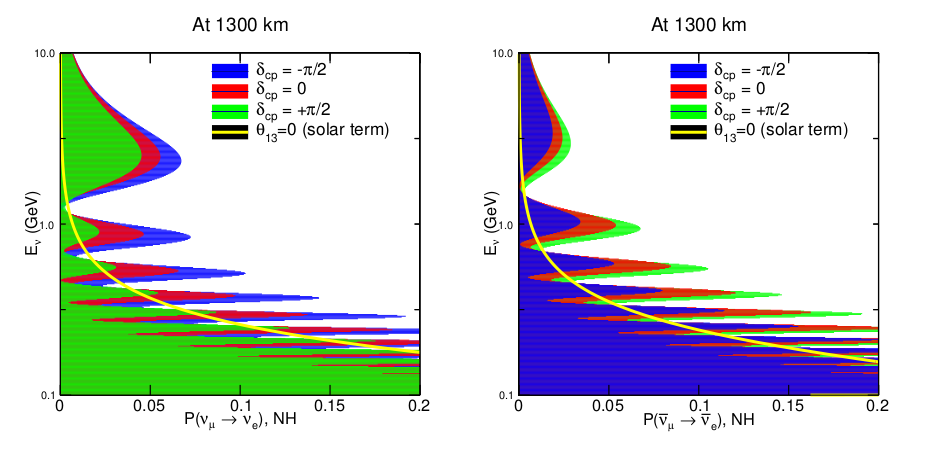
\includegraphics[width=0.98\textwidth, keepaspectratio=true]{figs/LBNF_oscProbability.png}
  \\$P(\nu_\mu \rightarrow \nu_e)$ at a baseline of 1300 km, as a function of neutrino energy. Left - neutrinos, right - antineutrinos. Figure is taken from the LBNF CDR draft, volume physics\cite{ref_LBNFdoc_volume-physics}
  \end{figure}
\end{frame}

\begin{frame}\frametitle{Available Experimental Results \cite{ref_PDG}}
  \scriptsize
  \begin{itemize}
    \item $sin^2(2\theta_{12})$=$0.846\pm0.021$
    \item $sin^2(2\theta_{23})$=$0.999^{+0.001}_{-0.018}$
    \item $sin^2(2\theta_{23})$=$1.000^{+0.000}_{-0.017}$
    \item ${\Delta}m^2_{21}$=$(7.53\pm0.18) \cdot 10^{-5} eV^2$
    \item ${\Delta}m^2_{32}$=$(2.44\pm0.06) \cdot 10^{-3} eV^2$ $\leftarrow$ if $m_3>m_2>m_1$
    \item ${\Delta}m^2_{32}$=$(2.52\pm0.07) \cdot 10^{-3} eV^2$ $\leftarrow$ if $m_1>m_2>m_3$
    \item CP-violation phase $\delta_{CP}$ - not measured
    \item mass hierarchy - not determined
  \end{itemize} 
\end{frame}


\begin{frame}\frametitle{Long Baseline Neutrino Facility (LBNF) Experimental Setup}
\scriptsize
\begin{figure}
\label{fig:LBNF_overallScheme}
\centering
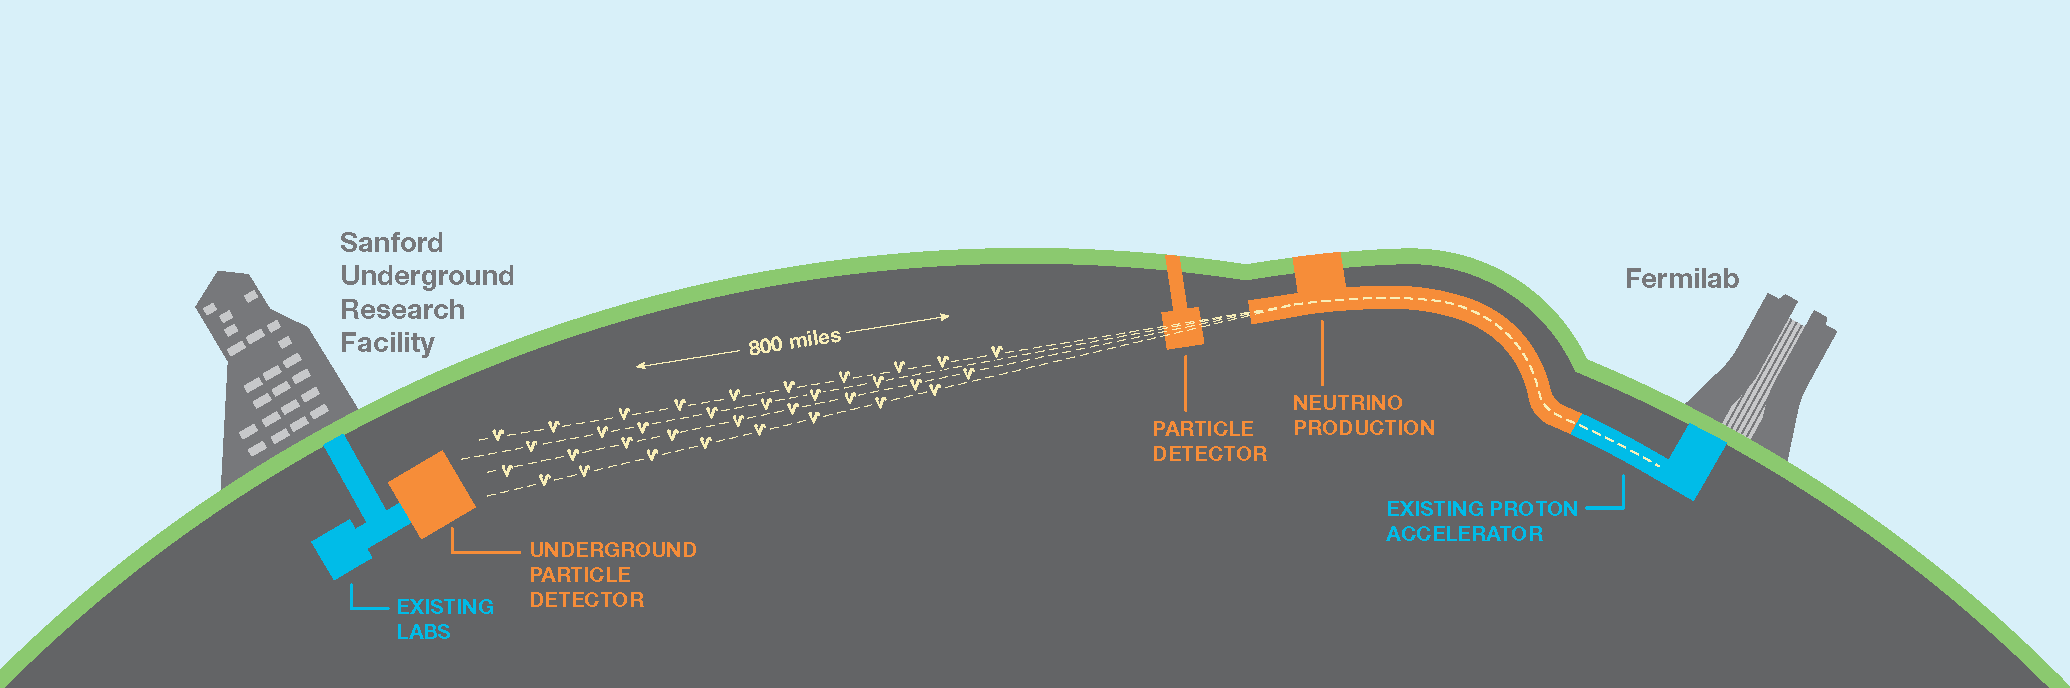
\includegraphics[width=0.95\textwidth, keepaspectratio=true]{figs/LBNF_overallScheme.png} 
\end{figure}
\begin{itemize}
  \item neutrino beam production system at FNAL, Illinois 
  \item near detector at FNAL, Illinois 
  \item far detector at SURF, South Dakota
\end{itemize}
\tiny
FNAL - Fermilab National Accelerator Laboratory, SURF - Sanford Underground Research Facility\\
Source of figure: \cite{ref_LBNFweb} 
\end{frame}

\begin{frame}
\begin{figure}
\label{fig:LBNF_FermilabAccComplex}
\centering
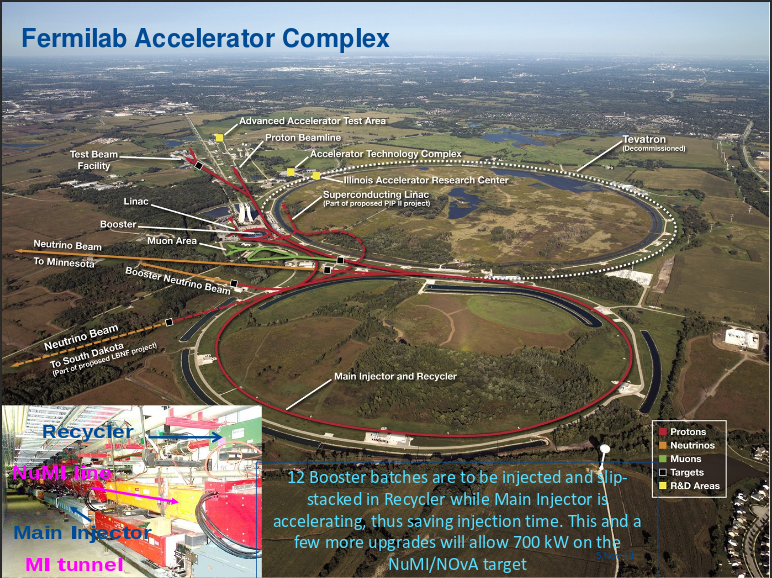
\includegraphics[width=0.95\textwidth, keepaspectratio=true]{figs/FermilabAccelerator.png}
\end{figure}
\end{frame}

\begin{frame}\frametitle{LBNF. Beam Production System}
\scriptsize
\begin{figure}
\label{fig:LBNF_nuBeam}
\centering
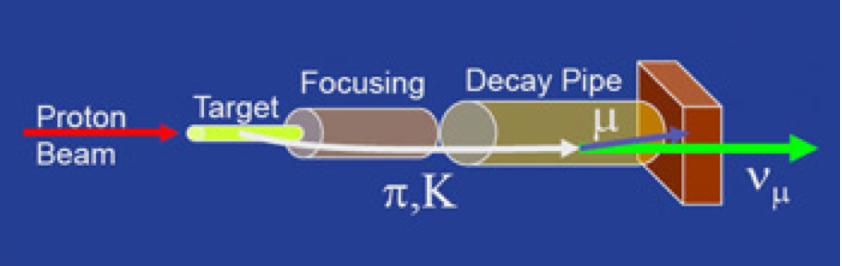
\includegraphics[width=0.45\textwidth, keepaspectratio=true]{figs/LBNF_nuBeam.png}  
\end{figure}
The neutrino beam production at the LBNF. Source of figure: \cite{ref_LBNFweb}\\
Pions (or kaons) are created: $p+p \rightarrow p+n+\pi^+$, $p+p \rightarrow p+\Delta^{++}+\pi^-$, $p+n \rightarrow p+p+\pi^-$, $p+n \rightarrow n+n+\pi^+$, $p+n \rightarrow p+\Delta^{-}+\pi^+$\\
And then decay: $\pi^+ \rightarrow \mu^+\nu_\mu$, $\pi^- \rightarrow \mu^-\bar{\nu_\mu}$, $K^+ \rightarrow \mu^+\nu_\mu$, $K^- \rightarrow \mu^-\bar{\nu_\mu}$\\
(Feynmann diagrams of these reactions are shown at the next slide)
\end{frame}

\begin{frame}\frametitle{LBNF. Pions and kaon creation and decay}
\scriptsize
\begin{figure}
\label{fig:pionAndKaonProductions}
\centering
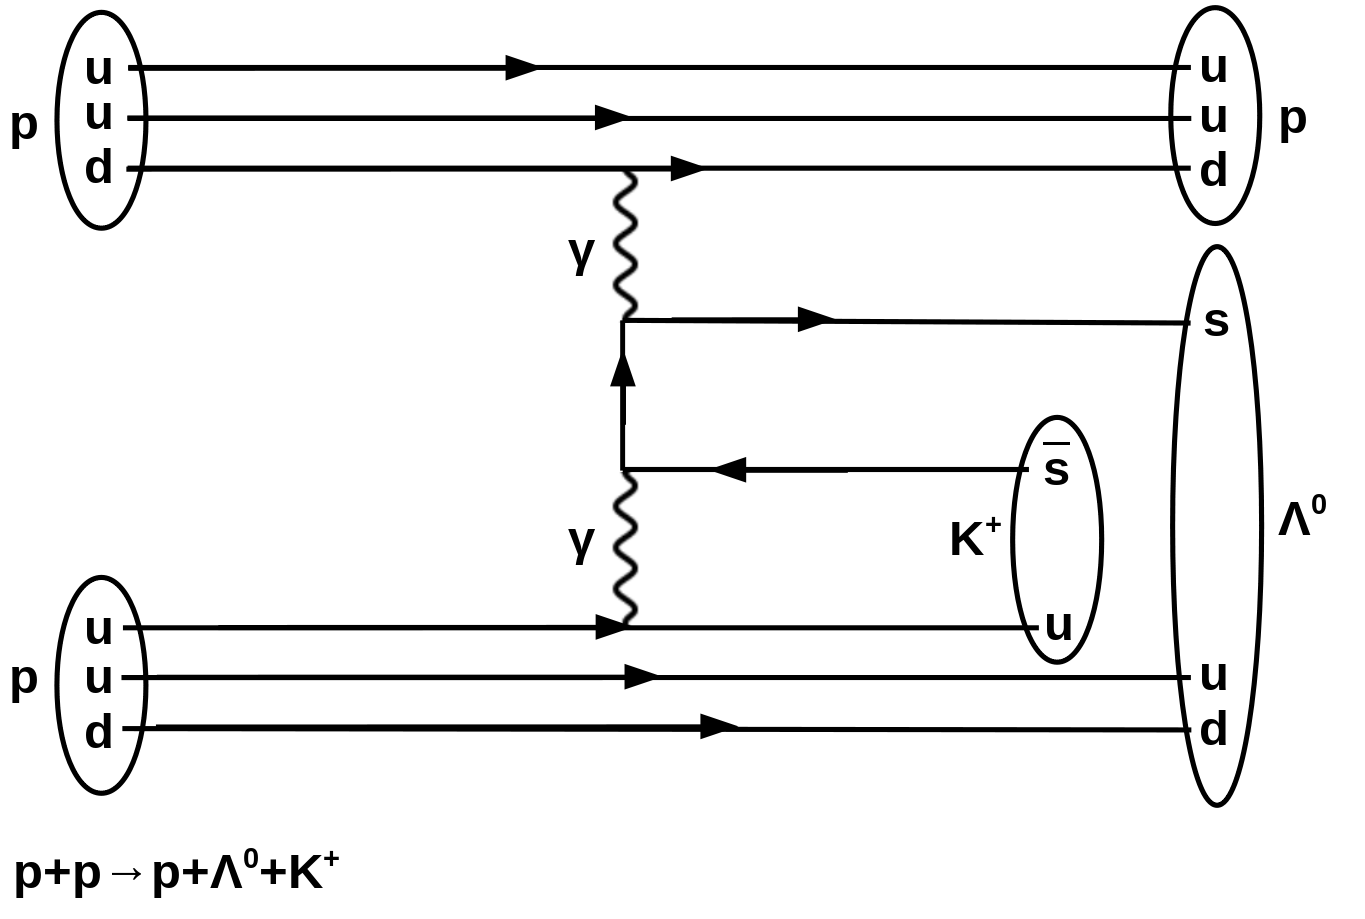
\includegraphics[width=0.48\textwidth, keepaspectratio=true]{figs/ppKaonProduction.png}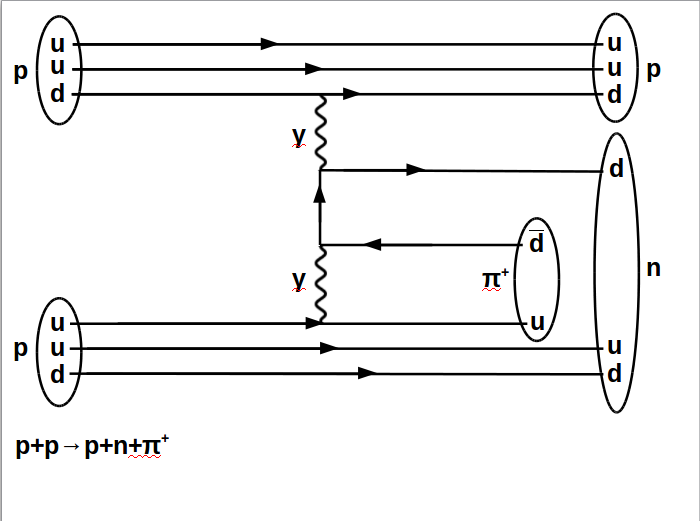
\includegraphics[width=0.48\textwidth, keepaspectratio=true]{figs/ppPionProduction.png}  
\end{figure}
\begin{figure}
\caption{Feynmann diagrams of charged pion and kaon decays to muon and muon antineutrino weakly through W-boson. Figures taken from \cite{ref_fig_pionandKaonDecays}.}
\label{fig:pionAndKaonDecays}
\centering
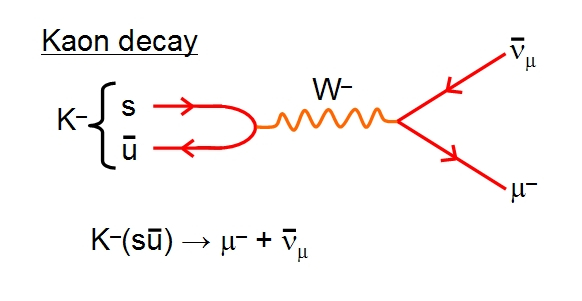
\includegraphics[width=0.45\textwidth, keepaspectratio=true]{figs/kaonDecay.jpg}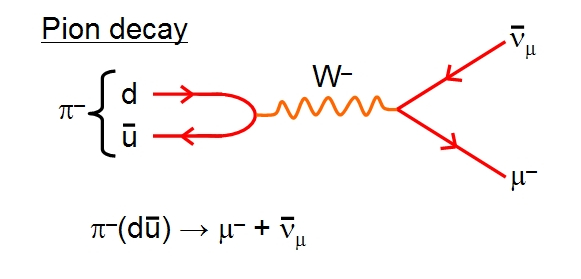
\includegraphics[width=0.45\textwidth, keepaspectratio=true]{figs/pionDecay.jpg} 
\end{figure}
\end{frame}

\begin{frame}\frametitle{LBNF. Near Detector}
\scriptsize
\begin{figure}
\label{fig:nearDetector}
\centering
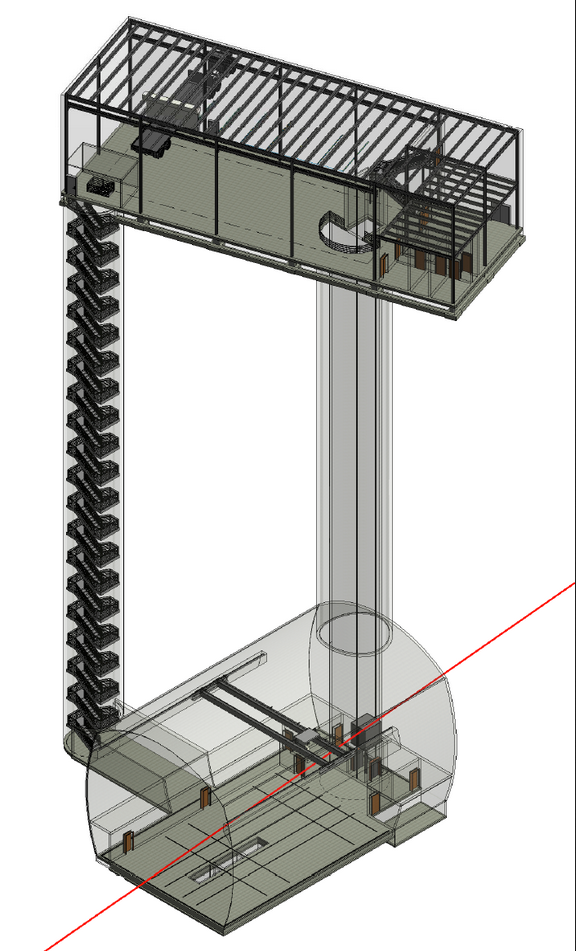
\includegraphics[width=0.25\textwidth, keepaspectratio=true]{figs/nearDetector_project.png}
\end{figure}
\scriptsize
Quoting the LBNF website \cite{ref_LBNFweb}, "The DUNE near detector will require LBNF to excavate and provision a cavern 200 ft (60 m) below grade on the Fermilab site and to construct a surface building directly above it. An elevator will provide the primary access between the two spaces; the stairway shown is planned for emergency egress. This complex will be constructed a minimum of 690 feet (210 m) downstream of the beamline target."
\end{frame}

\begin{frame}\frametitle{LBNF. Near Detector}
\scriptsize
\begin{figure}
\label{fig:nearDetector}
\centering
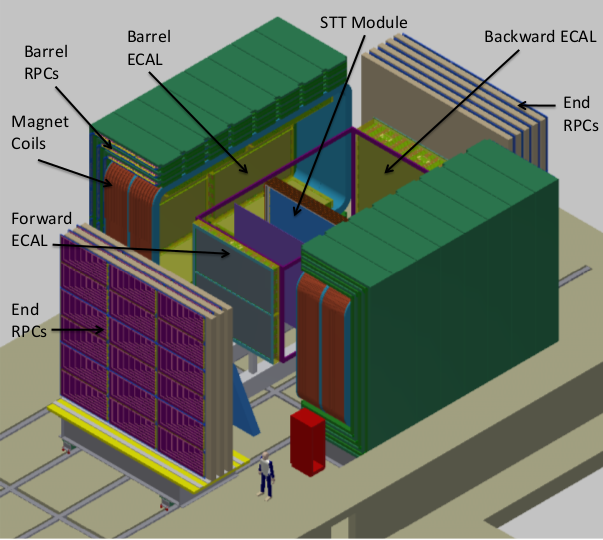
\includegraphics[width=0.50\textwidth, keepaspectratio=true]{figs/nearDetector.png}
\end{figure}
\scriptsize
The scheme of the near detector is shown at the fig. \ref{fig:nearDetector}. The detector will consist of central Straw-Tube Tracker (STT) modules, electromagnetic calorimeter (ECAL), magnet coils of 0.4T and muon identification system consisting of Resistive Plate Chamber (RPC) modules. The neutrinos would come from the bottom left corner of the picture, to the End RPCs.\\
\end{frame}

\begin{frame}\frametitle{LBNF. Near Detector Physics}
\scriptsize
\tiny
\begin{itemize}
  \item absolute flux measurement
  \item relative neutrino and antineutrino flux measurements
  \item flavor content of the neutrino source
  \item determination of the $E_\nu$-scale of neutrinos versus antineutrinos
  \item event-by-event measurements of NC interactions
  \item measurement of $\pi^0$, $\pi^\pm$, $K^\pm$, p, $K^0_S$ and $\Lambda$ in the NC and CC
%  \item "quasi-elastic and resonance measurements"
  \item nucleon structure, parton distribution functions and QCD studies
%  \item neutrino-argon interactions and nuclear effects
  \item precision measurements of electroweak physics
%  \item isospin physics and the Adler sum rule
%  \item measurement of the nuclean strangeness content
\end{itemize}

More specifically, the list of the physics measurements related to the neutrino oscillations to be performed by the Near Detector includes:
\begin{itemize}
  \item fluxes of $\nu_\mu$, $\bar{\nu_\mu}$, $\nu_e$ and $\bar{\nu_e}$. To distinguish between flavors, the measurement should rely on charged current interaction (fig. \ref{fig:MuonAndNeutronDecays}, middle and right) and measure the products of these interactions $\mu^-$, $\mu^+$, $e^-$, and $e^+$. (While the beam production system has the highest probability to produce muon neutrinos, the production of certain number electron neutrinos is also possible, for example, from charged kaon decays)
  \item $\nu_e$-$\bar{\nu_e}$ assymetries. For that, it's important not only distinguish between $\mu^\pm$ and $e^\pm$ but also between $e^-$ and $e^+$.
  \item the absolute $\nu_\mu$ and $\bar{\nu_\mu}$ fluxes need to be measured with $\simeq{3\%}$ precision in the neutrino energy range 0.5-8 GeV
  \item cross section of NC versus CC processes as a function of hadronic energy. NC is one of major backrounds which contribute to neutrino oscillation measurement
  \item yields of $\pi_0$ and photons. These particles are the most significant background to $\nu_e$ and $\bar{\nu_e}$ contamination
  \item fractions of the $\pi^\pm$ into the CC and the NC hadronic jets.    
\end{itemize} 
\end{frame}

\begin{frame}\frametitle{LBNF. SURF (Far Detector Site)}
\begin{figure}
\label{fig:farDetector_SURF1}
\centering
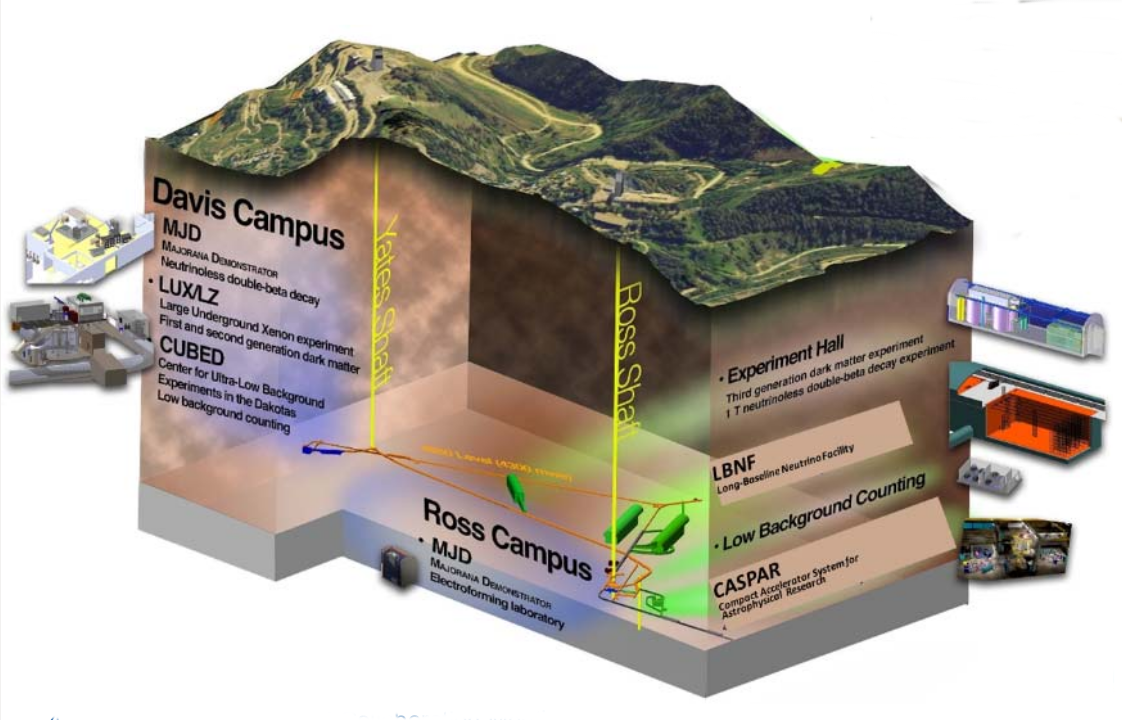
\includegraphics[width=0.98\textwidth, keepaspectratio=true]{figs/farDetector_SanfordUndergroundResearchFacility.png}
\end{figure}
\end{frame}

\begin{frame}\frametitle{LBNF. SURF (Far Detector Site)}
\begin{figure}
\label{fig:farDetector_SURF2}
\centering
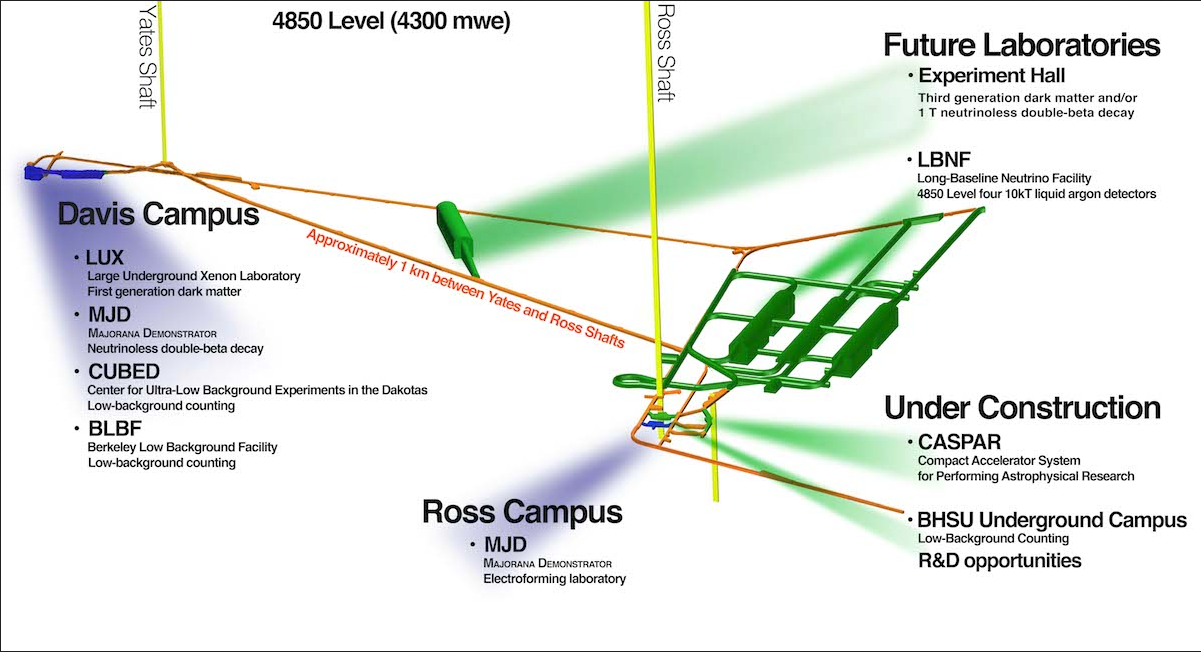
\includegraphics[width=0.98\textwidth, keepaspectratio=true]{figs/farDetector_wholeLab.png}
\end{figure}
\scriptsize
4 modules (15m x 12m x 58m, 10,000 tonnes of liquid argon each) placed into 4 caverns 1500 m underground. 5th cavern between two pairs - cryogenic equipment\\
\end{frame}

\begin{frame}\frametitle{LBNF. Far Detector. Liquid Argon Time Projection Chamber}
\begin{figure}
\label{fig:farDetector_TPC}
\centering
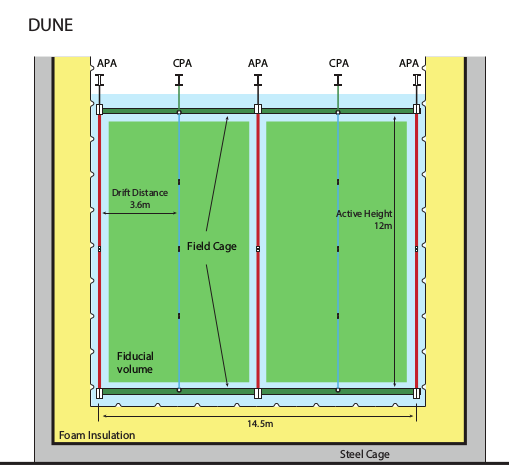
\includegraphics[width=0.75\textwidth, keepaspectratio=true]{figs/farDetector_TPC.png}
\end{figure}
\end{frame}

\begin{frame}\frametitle{LBNF Compared to the Other Experiments}
\tiny
  \begin{tabular}{|c|c|c|c|c|c|}
              & KEK (K2K) & NuMI & CNGS & T2K & LBNF (DUNE)\\ \hline
     location & Japan  & Illinois - & Switzerland - & Japan & Illinois - \\ 
              &        & Minnesota & Italy &  & South Dakota\\ \hline
     accelerator & KEK PS  & FNAL & CERN's SPS & J-PARC & FNAL\\ \hline
     time of oper. & 1999-2004  & 2005-2012 & 2006-2012 & 2010- & future \\ \hline 
     beam power  &  5 kW  & 300-350 kW  & 300 kW & 750 kW & 2000 kW\\ \hline 
     $E_p$  & 12 GeV & 120 GeV & 400 GeV & 30 GeV & 60-120 GeV\\ \hline 
     baseline  & 250 km & 735 km & 730 km & 295 km & 1300 km\\ \hline 
%                & KEK (K2K)   & NuMI                & CNGS                & T2K         & LBNF (DUNE)\\ \hline
     near        & (water ChD) & MINOS               & (muon               & ND280       & DUNE (FGD)\\  
     detector(s) & (FGD)       & (track. and scint.) & detector)           & INGRID      & \\ \hline 
     ND mass     & 1 kt (ChD)  & 0.98 kt             &                     &             & \\ \hline 
     far         & SuperK      & MINOS               & ICARUS (LAr)        & SuperK      & DUNE (LAr)\\  
     detector(s) & (water ChD) & track. and scint.   & OPERA (FGD)        & (water ChD) & \\ \hline 
     FD mass     & 50 kt       & 5.4 kt              & 0.76 kt (ICARUS)   & 50 kt       & 40 kt\\ 
                 &             &                     & 1.25 kt (OPERA)    &             & \\ \hline 
 \end{tabular}
\end{frame}

\begin{frame}\frametitle{LBNF. Status}
\scriptsize
\begin{itemize}
  \item Experiment is under development
  \item Conceptual Design Report (CDR) drafts are partially available
  \item First collaboration meeting took place on April 16th-18th, 2015
  \item Fermilab accelerator is available 
  \item Cavern for the near detector to be excavated
  \item Caverns for the far detector exist (former Homestake mine)
  \item far detector installation planned on 2021-2022
\end{itemize}
\end{frame}


\begin{frame}\frametitle{Conclusions}
  \scriptsize
  \begin{itemize}

     \item LBNF - long baseline neutrino oscillations experiment under development to be hosted by FNAL and SURF 
     \item Conceptual Design Report (CDR) drafts are partially available
     \item First collaboration meeting took place on April 16th-18th, 2015
     \item Collaboration of $>750$ people ($\sim$ 200 attended the 1st meeting on April 16th-18th of 2015)
     \item Expected parameters: baseline - 1300 km, beam power - 2 MW, far detector - 40kt of liquid argon
     \item Fermilab accelerator is available 
     \item Cavern for the near detector to be excavated
     \item Caverns for the far detector exist (former Homestake mine)
     \item plan: far detector installation in 2021-2022
     \item plan on precise measuments of $\theta_{12}$, $\theta_{23}$, $\theta_{13}$, $|\Delta{m_{12}}^2|$, $|\Delta{m_{31}}^2|$
     \item expected: to measure CP-violation phase $\delta_{CP}$ and $\nu$ mass hierarchy which never was measured before
     \item not expected: to measure absolute values of $\nu$ masses (different type of experiment would be needed)
  \end{itemize}
  \tiny
  * Paper and presentation for this comprehensive exam are available online: \cite{ref_my_paper}, \cite{ref_my_presentation}
\end{frame}

\begin{frame}[allowframebreaks]\frametitle{References}
\tiny
\begin{thebibliography}{1}
   \bibitem{ref_fig_StandardModel} website: http://www.isgtw.org/spotlight/go-particle-quest-first-cern-hackfest
   \bibitem{ref_Griffiths} David Griffiths "Introduction to Elementary Particles", Wiley-VCH; 2nd edition (October 13, 2008)
   \bibitem{ref_fig_neutrinoScattering}http://www.quora.com/What-particles-would-result-from-electron-neutrino-scattering
   \bibitem{ref_fig_NeutronDecay2} http://www.astroblogs.nl/2013/07/15/nucleosynthese-en-de-oerknal/bb-nucleo-11-neutron-decay/
   \bibitem{ref_LBNFdoc_volume-physics} LBNF CDR draft, physics: https://lbne.bnl.gov/tmp/volume-physics.pdf
   \bibitem{ref_PDG} K.A. Olive et al. (Particle Data Group), Chin. Phys. C, 38, 090001 (2014) 
   \bibitem{ref_LBNFweb} LBNF website: http://lbnf.fnal.gov/
   \bibitem{ref_fig_pionandKaonDecays} website: http://cronodon.com/Atomic/EWT.html
   \bibitem{ref_LBN_OscExpReview} G. J. Feldman, J. Hartnell, T. Kobayashi, A Review of Long-baseline Neutrino Oscillation Experiments, Advances in High Energy Physics 2013 (2013), 475749
   \bibitem{ref_my_paper} paper for this exam: https://github.com/eavdeeva/Comprehensive\_LBNF/blob/master/Main.pdf
   \bibitem{ref_my_presentation} this presentation: https://github.com/eavdeeva/Comprehensive\_LBNF/blob/master/presentation\_Comprehensive\_LBNF.pdf
   \bibitem{ref_Homestake} Bruce T. Cleveland et. al., Measurement of the Solar Electron Neutrino Flux with the Homestake Chlorine Detector, 1998 Astrophysical Journal 496 505
   \bibitem{ref_SuperK} C.W.Walter, The Super-Kamiokande Experiment, Prepared for inclusion in "Neutrino Oscillations: Present Status and Future Plans", J. Thomas and P. Vahle editors, World Scientific Publishing Company, 2008. This version is 12 pages in REVTeX4 two-column format
   \bibitem{ref_SNO} John N. Bahcall, Global Analysis of Solar Neutrino Oscillations Including SNO CC Measurement, JHEP 0108:014,2001
   \bibitem{ref_fig_SNOscheme} website: http://ase.tufts.edu/cosmos/print\_images.asp?id=37
   \bibitem{ref_wiki_NeutrinoDetectors} website: http://en.wikipedia.org/wiki/Neutrino\_detector
   \bibitem{ref_fig_MuonDecay} website: http://www.hep.ucl.ac.uk/~jpc/all/ulthesis/node9.html
   \bibitem{ref_fig_NeutronDecay} website: http://en.wikipedia.org/wiki/Neutron
   \bibitem{ref_LBNFdoc_volume-detectors} LBNF CDR draft, detectors: https://lbne.bnl.gov/tmp/volume-detectors.pdf
   \bibitem{ref_LBNF_collaborationMeeting} Agenda of the first LBNF collaboration meeting: https://indico.fnal.gov/conferenceOtherViews.py? view=standard\&confId=9740
   \bibitem{ref_fig_cosmicMuons} website: http://hardhack.org.au/book/export/html/2
   \bibitem{ref_KEK} M. Ieiri et al. . Proceedings of the 11th Symposium on Accelerator Science and Technology, SPring-8, Harima Science Garden City, Hyogo, Japan pages 377–379 (1997)
   \bibitem{ref_NuMI} K. Anderson et al. The NuMI Facility Technical Design Report. FERMILAB-DESIGN-1998-01 (1998)
   \bibitem{ref_CNGS} G. Acquistapace et al. The CERN neutrino beam to Gran Sasso (NGS). CERN-98-02, INFN-AE-98-05, CERN-YELLOW-98-02 (1998)
   \bibitem{ref_JPARC} K. Abe et al. (T2K Collaboration). The T2K Experiment. Nucl.Instrum.Meth. A659, 106–135 (2011). [1106.1238.]
   \bibitem{ref_aboutLAr} website Fermilab today: http://www.fnal.gov/pub/today/archive/archive\_2014/today14-10-09.html
\end{thebibliography}
\end{frame}

\begin{frame}
\huge
\begin{center}
BACKUP
\end{center}
\end{frame}

\begin{frame}\frametitle{Cosmic Shower and Muon Decay}
\begin{figure}
\caption{Cosmic shower induced by scattering of the incident cosmics proton of an air molecule. Charged and neutron pions are born in the reaction and then they further decay as $\pi^0 \rightarrow \gamma\gamma$, $\pi^+ \rightarrow \mu^+ + \nu_\mu$, $\pi^- \rightarrow \mu^- + \bar{\nu_\mu}$. Muon decay \cite{ref_fig_MuonDecay}(muon decays to electron, neutrino and antineutrino through W-boson}
\label{fig:cosmicMuons}
\centering
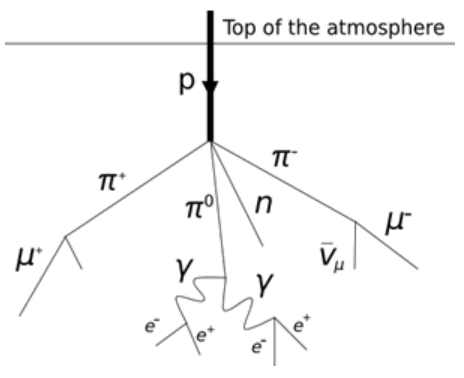
\includegraphics[width=0.35\textwidth, keepaspectratio=true]{figs/cosmicMuons.png}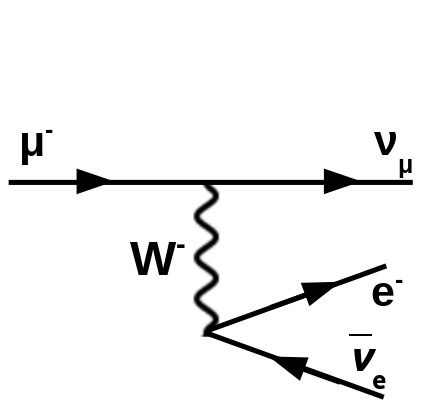
\includegraphics[width=0.35\textwidth, keepaspectratio=true]{figs/MuonDecay.png}
\end{figure}
\end{frame}

\begin{frame}\frametitle{Theory. Two Neutrinos Case}
  \scriptsize
  \begin{center}
  $\nu_1=\nu_{\mu}cos\theta-\nu_esin\theta$\\
  $\nu_2=\nu_{\mu}sin\theta+\nu_ecos\theta$\\
  \end{center}
  \begin{center}
  $\nu_1(t)=\nu_1(0)e^{\frac{-iE_1t}{\hbar}}$, $\nu_2(t)=\nu_2(0)e^{\frac{-iE_2t}{\hbar}}$ $\leftarrow$ from quantum mechanics\\
  \end{center}
  Suppose, at t=0 there were $\nu_e(0)=1$, $\nu_\mu(0)=0$\\
  Then: $\nu_1(0)=-sin\theta$, $\nu_2(0)=cos\theta$, $\nu_1(t)=-{sin\theta}e^{\frac{-iE_1t}{\hbar}}$, $\nu_2(t)=-{cos\theta}e^{\frac{-iE_2t}{\hbar}}$\\
  Therefore, we are getting the system:\\
  \begin{center}
  $-{sin\theta}e^{-{{iE_1t} \over \hbar}}=\nu_\mu(t)cos\theta-\nu_e(t)sin\theta$,\\
  $-{sin\theta}e^{-{{iE_2t} \over \hbar}}=\nu_\mu(t)sin\theta-\nu_e(t)cos\theta$\\
  \end{center}
  By solving this system for $\nu_e$ and $\nu_\mu$, one would get:\\
  \begin{center}
  $P_{\nu_e \rightarrow \nu_\mu}=|\nu_\mu(t)|^2=[{sin2\theta}sin{\frac{(E_1-E_2)t}{2\hbar}}]^2$,\\
  $P_{\nu_e \rightarrow \nu_e}=|\nu_e(t)|^2=1-[{sin2\theta}sin{\frac{(E_1-E_2)t}{2\hbar}}]^2$\\
  \end{center}
\end{frame}

\begin{frame}\frametitle{Theory. Two Neutrinos Case}
  \scriptsize
  \begin{center}
  $P_{\nu_e \rightarrow \nu_\mu}=|\nu_\mu(t)|^2=[{sin2\theta}sin{\frac{(E_1-E_2)t}{2\hbar}}]^2$,\\
  $P_{\nu_e \rightarrow \nu_e}=|\nu_e(t)|^2=1-[{sin2\theta}sin{\frac{(E_1-E_2)t}{2\hbar}}]^2$\\
  \end{center}
  Therefore, for freely travelling neutrinos, if $\nu_e$ was emmitted, at any point there is a certain probability to register $\nu_e$ or $\nu_\mu$ and those probablities change with time periodically, by $~[sin(At)]^2$ law. That's why the phenomenon is called the neutrino oscillations.
  Suppose momenta $p_1=p_2$. Then using $E^2=p^2{\cdot}c^2+m^2{\cdot}c^4$ and assuming $m_{1,2}c^2 \ll E_{1,2}$: \\
  \begin{center}
  $P_{\nu_e \rightarrow \nu_\mu}=|\nu_\mu(t)|^2=[{sin2\theta}sin{\frac{(E_1-E_2)t}{2\hbar}}]^2=[{sin2\theta}sin{\frac{(m_1^2-m_2^2)c^3}{4\hbar{E}}z}]^2$\\  
  \end{center}
\end{frame}

\begin{frame}\frametitle{Theory. Three Neutrinos Case (continued)}
  \tiny
  The probability amplitudes of neutrino mixing are defined by parameters of the $U_{PMNS}$ but, analogous to simplified two-neutrino case described above, the differences of squares of neutrino masses also contribute to the probability. There are two independent expressionce for squares of masses differences: ${\Delta}m_{12}^2 = m_1^2-m_2^2$ and ${\Delta}m_{32}^2 = m_3^2-m_2^2$. Mass differences were measured in other neutrino oscillation experiments but the ${\Delta}m_{12}^2$ and ${\Delta}m_{32}^2$ present in the equations evenly and therefore the signs of these expressions were not measured. If the masses order as $m_3 > m_2 > m_1$, it's called normal neutrino mass hierarchy because other fundamental particles orders in a way that later generation particles have higher masses than lower generation particles. If the masses order as $m_1 > m_2 > m_3$ it's called inverted neutrino mass hierarchy. The mixing angles $\theta_{12}$, $\theta_{23}$, $\theta_{13}$ and differences of squared masses $|{\Delta}m_{12}^2|$ and $|{\Delta}m_{32}^2|$ are measured and give $U_{PMNS}$ matrix form of\\
  \begin{center}
  $|U_{PMNS}| \sim
  \begin{pmatrix}
  0.8 & 0.5 & 0.2 \\ 0.5 & 0.6 & 0.6 \\ 0.2 & 0.6 & 0.8 \\
  \end{pmatrix}$\\
  \end{center}
  The CP-violating phase $\delta_{CP}$ is unknown.\\
  The analogous matrix for quark mixing, Cabibbo-Kobayashi-Maskawa (CKM) matrix $V_{CKM}$, is much more diagonal:\\
  \begin{center}
  $|V_{CKM}| \sim
  \begin{pmatrix}
  1 & 0.2 & 0.004 \\ 0.2 & 1 & 0.04 \\ 0.008 & 0.04 & 1 \\
  \end{pmatrix}$\\
  \end{center}
  One of the important questions in modern particle physics is why the quark mixing angles are so much smaller than neutrino mixing angles and the other important question is whether there is any relationship between quark and neutrino mixing matrices.\\
\end{frame}

\begin{frame}
\begin{figure}
\label{fig:LBNF_FermilabAccComplex}
\centering
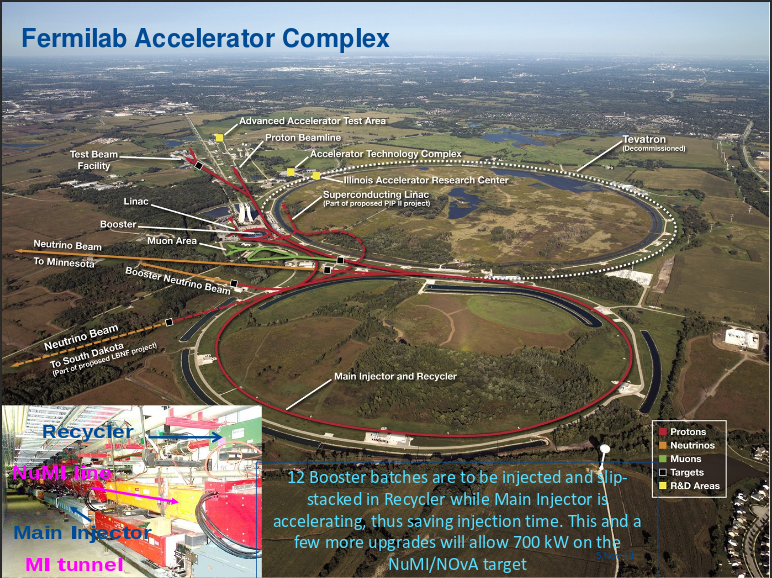
\includegraphics[width=0.95\textwidth, keepaspectratio=true]{figs/FermilabAccelerator.png}
\end{figure}
\end{frame}

\begin{frame}\frametitle{LBNF. Near Detector Physics}
\scriptsize
\tiny
\begin{itemize}
  \item absolute flux measurement
  \item relative neutrino and antineutrino flux measurements
  \item flavor content of the neutrino source
  \item determination of the $E_\nu$-scale of neutrinos versus antineutrinos
  \item event-by-event measurements of NC interactions
  \item measurement of $\pi^0$, $\pi^\pm$, $K^\pm$, p, $K^0_S$ and $\Lambda$ in the NC and CC
%  \item "quasi-elastic and resonance measurements"
  \item nucleon structure, parton distribution functions and QCD studies
%  \item neutrino-argon interactions and nuclear effects
  \item precision measurements of electroweak physics
%  \item isospin physics and the Adler sum rule
%  \item measurement of the nuclean strangeness content
\end{itemize}

More specifically, the list of the physics measurements related to the neutrino oscillations to be performed by the Near Detector includes:
\begin{itemize}
  \item fluxes of $\nu_\mu$, $\bar{\nu_\mu}$, $\nu_e$ and $\bar{\nu_e}$. To distinguish between flavors, the measurement should rely on charged current interaction (fig. \ref{fig:MuonAndNeutronDecays}, middle and right) and measure the products of these interactions $\mu^-$, $\mu^+$, $e^-$, and $e^+$. (While the beam production system has the highest probability to produce muon neutrinos, the production of certain number electron neutrinos is also possible, for example, from charged kaon decays)
  \item $\nu_e$-$\bar{\nu_e}$ assymetries. For that, it's important not only distinguish between $\mu^\pm$ and $e^\pm$ but also between $e^-$ and $e^+$.
  \item the absolute $\nu_\mu$ and $\bar{\nu_\mu}$ fluxes need to be measured with $\simeq{3\%}$ precision in the neutrino energy range 0.5-8 GeV
  \item cross section of NC versus CC processes as a function of hadronic energy. NC is one of major backrounds which contribute to neutrino oscillation measurement
  \item yields of $\pi_0$ and photons. These particles are the most significant background to $\nu_e$ and $\bar{\nu_e}$ contamination
  \item fractions of the $\pi^\pm$ into the CC and the NC hadronic jets.    
\end{itemize} 
\end{frame}


\end{document}
